\section{Implemented Features}
	
\subsection{Basic Interaction}
	\label{sec-basic-interaction}
	In the following, a short overview over the basic functions of the application shall be given.
	
	\paragraph{Project and Document management}
	% Project organization
		All works created by the user are organized on two hierarchy levels:

		\begin{description}	
		\item[Documents]
			are representations of exactly one design each.
			Their most notable trait is the association with a schematic visualization, which can be edited by the user.
			Documents do not exist on their own but rely on the existence of a project to be contained in.
			Any circuit described by a document carries the documents name and is referred to as a \emph{module}.
		\item[Projects]
			form a collection of documents and an associated component hierarchy.
		% Saving and loading via JSON
			They can be saved to and loaded from a persistent storage medium, where the project itself forms a folder with all contained documents as separate \gls{json} files.
		\end{description}
	
		While it is possible to discard unsaved projects, it is at the time of writing not implemented to delete documents via the \gls{ui}.
		This effect can however be achieved by removing the corresponding \gls{json} file from the projects folder and re-loading the project.\footnote{
			Due to time restrictions, there is a set of similar usability functions that were not present at the time of writing.
			Since most of them could be emulated by simply editing a \gls{json} file, they were considered low priority.
		}
	
	% Managing the component hierarchy
	\paragraph{The Component Hierarchy}
		As described in section \ref{sec-model-design}, a hierarchy is used for the organization of component types.
		These are available as \emph{descriptor files}, which will be detailed in section \ref{sec-user-defined-components}.
		Also, categories are available, to allow arranging component types hierarchically as the user desires.  
		It is possible to load provided descriptor files. 
		The contained component descriptors will be sorted as child items of the currently selected category or the implicitly available root item, if no category is selected.
		By expanding entries of component types, information about contained elements like ports, configuration bits and functional behaviour description can be accessed.

	% Creating Schematics
	\paragraph{Creating Schematics}
		After the creation of a document, component types can be dragged from the component hierarchy view to create an instance of this exact type in the schematic.
		The newly spawned instance will automatically be given a valid and unique name.
		Each document tab offers buttons to add in- and output \emph{module ports} that connect the module described by the document to the outside world.
		All placed component instances and module ports can be connected by wires to form a complete circuit design.
	
\subsection{User-Defined Components}
	\label{sec-user-defined-components}
	
	As discussed in section \ref{sec-model-design}, it was decided to allow users to create their own component types.
	Writing a \gls{json} file that represents a certain component turned out to be quite feasible, especially, when already provided with a template which only needs to be filled in.
	
	\paragraph{A Minimal Example}
		To illustrate the process of	creating a custom component type, a rather minimal example is shown in listing \ref{code-minimal-descriptor}.
		It describes a \glslink{lut}{2-LUT} with the input ports $x0$, $x1$, the output port $y$ and four configuration bits $c_0 \cdots c_3$.
		The latter are created in line 11 by declaring the existence of a group of configuration bits called $c$, having four members.
		When loading the descriptor file, \emph{q2d} will expand this notation into separate configuration bits.
		It was deemed useful to use this style of notation to be able to cope with larger amounts of configuration bits, contrary to declaring each bit explicitly.
		Given the case that certain bits carry a specific semantic meaning, they still can be put into groups appropriately.
		Note that the \gls{cbd} is specified as a set of clauses.
		There are other ways of specifying the \glspl{pcbd} of a component, which will be discussed in section \ref{sec-functional-behaviour-spec}.

	\includecode[json]{sources/descriptor-minimal.json}{A minimal component descriptor file}{code-minimal-descriptor}

\subsection{Generation of Circuit Symbols}
	\label{sec-symbol-generation}
	
	While testing the application, it has been found, that manually creating component symbols is quite time-consuming and users prefer achieving fast results over customizing their created component types.
	To speed up the workflow and relief the user of unnecessary side-tasks, it was found desirable to automatically create a default component symbol for each component type.
	
	\paragraph{Description of Automatically Generated Circuit Symbols}
	Important elements for generating a circuit symbol are the component's ports, type and instance name.
	The latter is generated from the type name upon instantiation by appending an underscore and an incremental zero-based index.
	
	\begin{figure}
		\centering
		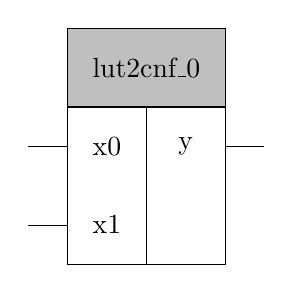
\begin{tikzpicture}

% instance name section
\filldraw[fill=lightgray] (0,2) rectangle (2,3);
\node (instancename) at (1,2.5) {lut2cnf\_0};

% input port section
\draw (0,0) rectangle (1, 2);
\node (portX0) at (0.5, 1.5) {x0};
\node (portX1) at (0.5, 0.5) {x1};
\draw (-0.5, 1.5) -- (0, 1.5);
\draw (-0.5, 0.5) -- (0, 0.5);


% output port section
\draw(1, 0) rectangle (2, 2);
\node (portY) at (1.5, 1.5) {y};
\draw (2, 1.5) -- (2.5, 1.5);

\end{tikzpicture} 
		\caption{An automatically generated component symbol}
		Based on listing \ref{code-minimal-descriptor}
		\label{fig-generated-symbol}
	\end{figure}
	
	Figure \ref{fig-generated-symbol} shows the subdivision of the symbol in three main areas.
	On the top, the instance name is centred, while the left side contains all input ports, and output ports are positioned to the right.
	The position of the port symbols is calculated during the creation of the circuit symbol and added to the component descriptor.
	It is not required to specify port positions in the descriptor file, as long as no custom symbol is used.
	
	\paragraph{User-Specified Circuit Symbols}
	Sometimes, it feels more convenient to the user to define their own symbol for certain component types, either because they are accustomed to them or because they want to convey additional information by visual means.
	This can be achieved by modifying the descriptor file.
	It is only required:
	
	\begin{itemize}	
		\item to add the property \texttt{symbolFile}, which specifies the location of the \gls{svg}-file containing the circuit symbol relative to the descriptor files location, and
		
		\item to extend the port descriptors by the positions, where to place the port symbols in the schematic.
		They are specified as a cartesian coordinates relative to the origin of the specified symbol file
	\end{itemize}
	
	An example can be found in listing \ref{code-modified-descriptor}.
	Note that the unaffected sections \texttt{name}, \texttt{configBits} and \texttt{functions} have been shortened to focus on the relevant changes.
	
	\includecode[json]{sources/descriptor-modified.json}{A descriptor file with a custom circuit symbol}{code-modified-descriptor}	
	
\subsection{Methods for Specifying Functional Behaviour}
	\label{sec-functional-behaviour-spec}
	
	While working with \emph{q2d}, it may become necessary to specify formulae.
	Two common examples are the \glspl{pcbd} contained in component descriptors and the specification of the target behaviour.
	Both cases shall be examined further in the paragraphs below.	
	
	\paragraph{General Considerations}
		Any formulae are specified in propositional logic.
		From a user's perspective, all behaviour is input as a list of strings.
		The elements of this list are treated as if they were conjuncted.
		Depending on the context, the set of valid variables may vary.
		
		For the convenience of users, different notations for logical operators are allowed.
		It is possible to either use symbols or mnemonics.\footnote{
			The recognition of mnemonics is case-sensitive.
			This might change in the future.
		}
		They are listed in table \ref{tab-logical-operators}.
		
		\begin{table}
			\centering
			\begin{tabular}{|r|crclc|}
				\hline
				Operator		& Type	& \multicolumn{3}{c}{Symbols}			& Mnemonic		\\
				\hline
				Negation		& prefix	& \textasciitilde \-	& \emph{or}	& !	& \texttt{not}	\\
				Conjunction	& infix	& \&	 				& \emph{or} 	& *	& \texttt{and}	\\
				Disjunction	& infix	& $|$ 				& \emph{or} 	& +	& \texttt{or}	\\
				Negated Conjunction	& infix & \multicolumn{3}{c}{\emph{(none)}}	& \texttt{nand}	\\
				Negated Disjunction	& infix	& \multicolumn{3}{c}{\emph{(none)}}	& \texttt{nor}	\\
				Exclusive Disjunction	&infix	& \multicolumn{3}{c}{\^}	& \texttt{xor}	\\
				Negated Exclusive Disjunction	&infix	& \multicolumn{3}{c}{\emph{(none)}}	& \texttt{xnor}	\\
				\hline
			\end{tabular}
			\caption{Overview of Logical Operator Notations in \emph{q2d}}
			\label{tab-logical-operators}
		\end{table}			
	
	\paragraph{Notation Styles}
		It is possible to use a clause notation like
		\begin{equation}
			\begin{aligned}
			&[ x, !y, z ] \\
			&[ x, y, !z ]
			\end{aligned}
		\label{eqn-styles-cnf}
		\end{equation}
		In this case, square brackets are used to delimit the clause, while commas separate the terms from each other.
		Unlike strict \gls{cnf}, a clause may not only contain literals but whole boolean expressions.
		
		The clauses of equation \ref{eqn-styles-cnf} could be re-written into a single expression:
		\begin{equation}
			(x\,|\,!y\,|\,z) \& (x\,|\,y\,|\,!z)
		\end{equation}
		
		As another often convenient alternative one might specify a boolean equation:
		\begin{equation}
			a = (b\ \text{or}\ c)\ \text{and}\ \text{not}\ d
		\label{eqn-styles-equation}
		\end{equation}
		Any non-\gls{cnf} style allows the usage of the equality operator and parenthesis to express precedence.
		The example in equation \ref{eqn-styles-equation} may be transcribed as
		\begin{equation}
			a \Leftrightarrow \left( b \vee c \right) \wedge \left(\neg d \right)
		\end{equation}
		
		It was shown in equation \ref{eqn-resolve-equivalence} how the equivalence can be resolved.
		The clause notation is mainly found in descriptor files.
		Each function represents one clause and all functions combined create a complete \gls{cnf} specification due to the line conjunction behaviour mentioned before.
		For most humans though, it feels more intuitive to specify boolean formulae, which results in this version being frequently used for specifying target formulae.
		
	
	\paragraph{\Glspl{cbd} in Descriptor Files}
		When creating component descriptors, it is often necessary to express the behaviour of a component.
		For that purpose, the descriptor files contain a \emph{functions}-section. 
		Within these functions, there is only a limited set of valid variables:
		\begin{description}
			\item[ports] represented by their respective names as provided in the \emph{ports}-section, as shown in listing \ref{code-minimal-descriptor}, lines 3 to 8.
			\item[configuration bits] that are named by taking the respective bit group name, adding an underscore and a corresponding incremental 0-based index number.
		\end{description}
		
	\paragraph{Target Formulae for SAT-solving}
		A target formula requires a module to be applied on.
		Any module interface name is a valid variable within the target function.\footnote{
			All releases of the application, up to the time of writing, accept	the full identifier of any component port as a variable as well.
			This behaviour seems to have no benefits regarding productive use so far, but proved useful for debugging. 
		}